\documentclass[11pt]{article}

\usepackage{mathtools}
\usepackage{amssymb}
\usepackage{amsmath}
\usepackage{amsthm}
\usepackage{hyperref}
\usepackage{microtype}
\usepackage{graphicx}
\usepackage{blkarray}
\graphicspath{ {./img/} }

\setlength{\parindent}{0cm}
\let\emptyset\varnothing

\title{\textbf{CSCI/MATH 2113 Discrete Structures} \\ 7.2 Computer Recognition: Zero-One Matrices and Directed Graphs}
\author{Alyssa Motas}

\begin{document}

    \maketitle

    \pagebreak

    \tableofcontents

    \pagebreak

    \section{Relation Composition}

    If \(A,B\) and $C$ are sets with \(R_1 \subseteq A \times B\) and \(R_2 \subseteq B \times C\), then the \emph{composite relation} \(R_1 ; R_2\) is a relation from $A$ to $C$ defined by \[R_1 ; R_2 = \{(x,z) \mid x \in A, z \in C, \exists y \in B \text{ with } (x,y) \in R_1, (y,z) \in R_2\}.\]

    \subsection{Example}

    Suppose that \(A = \{1,2,3,4\}\), \(B = \{w,x,y,z\}\), and \(C = \{5,6,7\}\) where
    \begin{align*}
        R_1 &= \{(1,x),(2,x),(3,y),(3,z)\} \subseteq A \times B \\
        R_2 &= \{(w,5),(x,6)\} \subseteq B \times C \\
        R_3 &= \{(w,5), (w,6)\} \subseteq B \times C
    \end{align*}
    Then we have \[R_1;R_2 = \{(1,6),(2,6)\}\] and \[R_1;R_3 = \emptyset.\]

    \subsection{Theorem}

    Let \(A,B,C\) and $D$ be sets with \(R_1 \subseteq A \times B\), \(R_2 \subseteq B \times C\), and \(R_3 \subseteq C \times D.\) Then \(R_1;(R_2;R_3) = (R_1;R_2);R_3.\)

    \begin{proof}
        If \((a,d) \in R_1;(R_2;R_3)\), then there is an element \(b \in B\) with \((a,b) \in R_1\) and \((b,d) \in (R_2;R_3)\). Also, \((b,d) \in (R_2;R_3) \Rightarrow (b,c) \in R_2\) and \((c,d) \in R_3\) for some \(c \in C\). Then \((a,b) \in R_1\) and \((b,c) \in R_2 \Rightarrow (a,c) \in R_1;R_2\). Finally, \((a,c) \in R_1;R_2\) and \((c,d) \in R_3 \Rightarrow (a,d) \in (R_1;R_2);R_3\), and \(R_1;(R_2;R_3) \subseteq (R_1;R_2);R_3\). The opposite inclusion follows by similar reasoning.
    \end{proof}

    \subsection{Powers of a relation}

    Given a set $A$ and a relation $R$ on $A$, we define the \emph{powers} of $R$ recursively by 
    \begin{enumerate}
        \item[(a)] \(R^1 = R;\)
        \item[(b)] for \(n \in \mathbb{Z}^+, R^{n+1} = R;R^n.\)  
    \end{enumerate}

    \emph{Example.} Suppose that \(A = \{1,2,3,4\}\) and \(R = \{(1,2),(1,3),(2,4),(3,2)\}\). Then we have
    \begin{align*}
        R^2 &= \{(1,4),(1,2),(3,4)\} \\
        R^3 &= \{(1,4)\} \\
        R^n &= \emptyset \text{ for } n \leq 4.
    \end{align*}

    \section{Zero-one matrices}

    An \(m \times n\) \emph{zero-one matrix} \(E = (e_{ij})_{m \times n}\) is a rectangular array of numbers arranged in $m$ rows and $n$ columns, where each \(e_{ij}\), for \(1 \leq i \leq m\) and \(1 \leq j \leq n\), denotes the entry in the $i$th row and $j$th column of $E$, and each such entry is 0 or 1. 
    
    \vspace{1em}

    \emph{Example.} The matrix 
    \begin{equation*}
        E = \begin{bmatrix}
            1 & 0 & 0 & 1 \\
            0 & 1 & 0 & 1 \\
            1 & 0 & 0 & 0
        \end{bmatrix}
    \end{equation*}
    is a \(3 \times 4\) (0,1)-matrix where, for example, \(e_{11} = 1, e_{23} = 0,\) and \(e_{31} = 1.\)

    \vspace{1em}

    \(0\) is the matrix such that \(0_{i,j} = 0.\) And \(1\) is the matrix such that \(1_{i,j} = 1.\) \(I_n\) is the identity matrix where 
    \begin{equation*}
        (I_n)_{i,j} = S_{i,j} = \begin{cases}
            1 \quad \text{ if } i = j \\ 0 \quad \text{ if } i \neq j
        \end{cases}
    \end{equation*}

    If $M$ is a matrix then \(M^{tr}\) is \[(M^{tr})_{i,j} = M_{j,i}\]

    We think of 0 and 1 as truth values and of \(\cdot\) (multiplication) as conjunction and of + (addition) as disjunction. This means that
    \begin{align*}
        0 \cdot 0 = 0 && 0 + 0 = 0 \\
        0 \cdot 1 = 0 && 0 + 1 = 1 \\
        1 \cdot 0 = 0 && 1 + 0 = 1 \\
        \underbrace{1 \cdot 1 = 1}_\text{logical ``and''} && \underbrace{1 + 1 = 1}_\text{logical ``or''}
    \end{align*}

    We use these operations when multiplying matrices.

    \vspace{1em}

    \emph{Example.}

    \begin{align*}
        &\begin{bmatrix}
            0 & 1 \\ 1 & 0
        \end{bmatrix} \begin{bmatrix}
                        0 & 1 \\ 1 & 0
                      \end{bmatrix} = \begin{bmatrix}
                                        1 & 0 \\ 0 & 1
                                    \end{bmatrix} = I_2 \\
        &\begin{bmatrix}
            1 & 1 \\ 1 & 0
        \end{bmatrix} \begin{bmatrix}
                        1 & 0 \\ 1 & 0
                    \end{bmatrix} = \begin{bmatrix}
                                    1 & 0 \\ 1 & 0
                                \end{bmatrix}
    \end{align*}
    As well as multiplication, we define another operation on matrices.

    Let $M$ and $N$ be \((0,1)\)-matrices of the same size. Then \(M \cap N\) is defined as \[(M \cap N)_{i,j} = M_{i,j} \cdot N_{i,j}.\]

    \vspace{1em}

    \emph{Example.}
    \begin{equation*}
        \begin{bmatrix}
            1 & 0 \\ 1 & 0
        \end{bmatrix} \cap \begin{bmatrix}
                                1 & 1 \\ 0 & 0
                            \end{bmatrix} = \begin{bmatrix}
                                                1 & 0 \\ 0 & 0
                                            \end{bmatrix}
    \end{equation*}
 
    \vspace{1em}

    Let $M$ and $N$ be \((0,1)\)-matrices of the same size. Then \[M \leq N\] if \(M_{i,j} \leq N_{i,j}\) for all \(i,j\). In this case, we say that $M$ \emph{precedes} $N$.

    \vspace{1em}

    \emph{Examples.}
    \begin{align*}
        \begin{bmatrix}
            1 & 0 \\ 0 & 0
        \end{bmatrix} &\leq \begin{bmatrix}
                                1 & 1 \\ 0  & 0
                            \end{bmatrix} \\
        \begin{bmatrix}
            1 & 0 \\ 0 & 0
        \end{bmatrix} &\nleq \begin{bmatrix}
                                0 & 0 \\ 0 & 1
                            \end{bmatrix} \\
        \begin{bmatrix}
            1 & 0 \\ 0 & 0
        \end{bmatrix} &\ngeq \begin{bmatrix}
                                0 & 0 \\ 0 & 1
                            \end{bmatrix}
    \end{align*}

    \subsection{Relation matrices}

    Suppose we have \(A = \{1,2,3,4\}\), \(B = \{w,x,y,z\}\), \(C = \{5,6,7\}\), \(R_1 = \{(1,x),(2,x),(3,y),(3,z)\}\), and \(R_2 = \{ (w,5), (x,6) \}\). The matrix for \(R_1, R_2\) is

    \begin{equation*}
        M(R_1) = \begin{blockarray}{ccccc}
                    & w & x & y & z \\
                    \begin{block}{c[ cccc ]}
                        1 & 0 & 1 & 0 & 0 \\
                        2 & 0 & 1 & 0 & 0 \\
                        3 & 0 & 0 & 1 & 1 \\
                        4 & 0 & 0 & 0 & 0 \\
                    \end{block}
                \end{blockarray} \qquad M(R_2) = \begin{blockarray}{cccc}
                    & 5 & 6 & 7 \\
                    \begin{block}{c [ccc]}
                        w & 1 & 0 & 0 \\
                        x & 0 & 1 & 0 \\
                        y & 0 & 0 & 0 \\
                        z & 0 & 0 & 0 \\
                    \end{block}
                \end{blockarray}
    \end{equation*}
    We have \[M(R_1;R_2) = M(R_1) \cdot M(R_2).\] So to figure out what the matrix for \(R_1;R_2\) is, it suffices to multiply the matrices for \(R_1\) and \(R_2\).

    \begin{equation*}
        M(R_1;R_2) = \begin{bmatrix}
                        0 & 1 & 0 & 0 \\
                        0 & 1 & 0 & 0 \\
                        0 & 0 & 1 & 1 \\
                        0 & 0 & 0 & 0
                    \end{bmatrix} \cdot \begin{bmatrix}
                                            1 & 0 & 0 \\
                                            0 & 1 & 0 \\
                                            0 & 0 & 0 \\
                                            0 & 0 & 0
                                        \end{bmatrix} = \begin{bmatrix}
                                                            0 & 1 & 0 \\
                                                            0 & 1 & 0 \\
                                                            0 & 0 & 0 \\
                                                            0 & 0 & 0
                                                        \end{bmatrix}
    \end{equation*}

    \subsection{Theorem}

    Let $A$ be a set with \(|A| = n \leq 1\), $R$ be a relation on $A$, and $M$ be the matrix for $R$. Then 
    \begin{enumerate}
        \item $R$ is reflexive if and only if \(I_n \leq M\).
        \item $R$ is symmetric if and only if \(M = M^{tr}\).
        \item $R$ is transitive if and only if \(M^2 \leq M\).
        \item $R$ is antisymmetric if and only if \(M \cap M^{tr} \leq I_n\).
    \end{enumerate}

    \section{Directed graphs}

    Let $V$ be a finite nonempty set. A \emph{directed graph} (or \emph{digraph}) $G$ on $V$ is made up of the elements of $V$, called \emph{vertices} or \emph{nodes} of $G$, anda  subset $E$, of \(V \times V\), that contains the (\emph{directed}) \emph{edges}, or \emph{arcs}, of $G$. The set $V$ is called the \emph{vertex set} of $G$, and the set $E$ is called the \emph{edge set}. We then write \(G = (V,E)\) to denote the graph.

    \vspace{1em}

    If \(a,b \in V\) and \((a,b) \in E\), then there is an edge from $a$ to $b$. Vertex $a$ is called the \emph{origin} or \emph{source} of the edge, with $b$ the \emph{terminus}, or \emph{terminating vertex}, and we say that $b$ is \emph{adjacent from a} and that $a$ is \emph{adjacent} to $b$. In addition, if \(a \neq b\), then \((a,b) \neq (b,a).\) An edge of the form \((a,a)\) is called a \emph{loop} at $a$.

    \pagebreak

    \emph{Example.} Suppose that \(V = \{1,2,3,4,5\}\) and \(E = \{(1,1),(1,2),(1,4),(3,2)\}\). Then
    \begin{center}
        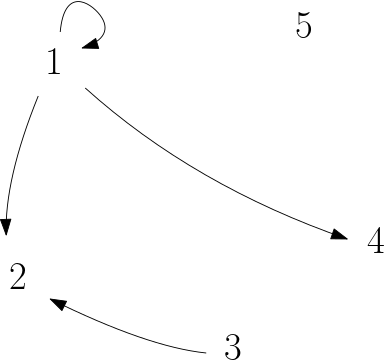
\includegraphics[width=5cm]{graph1.png}
    \end{center}

    We can interpret a relation on a set $A$ as a directed graph.

    \vspace{1em}

    \emph{Example.} Suppose that \(A = \{1,2,3,4\}\) and \(R = \{(1,1),(1,2),(2,3),(3,2),(3,3),(3,4),(4,2)\}\). Then we have 

    \begin{center}
        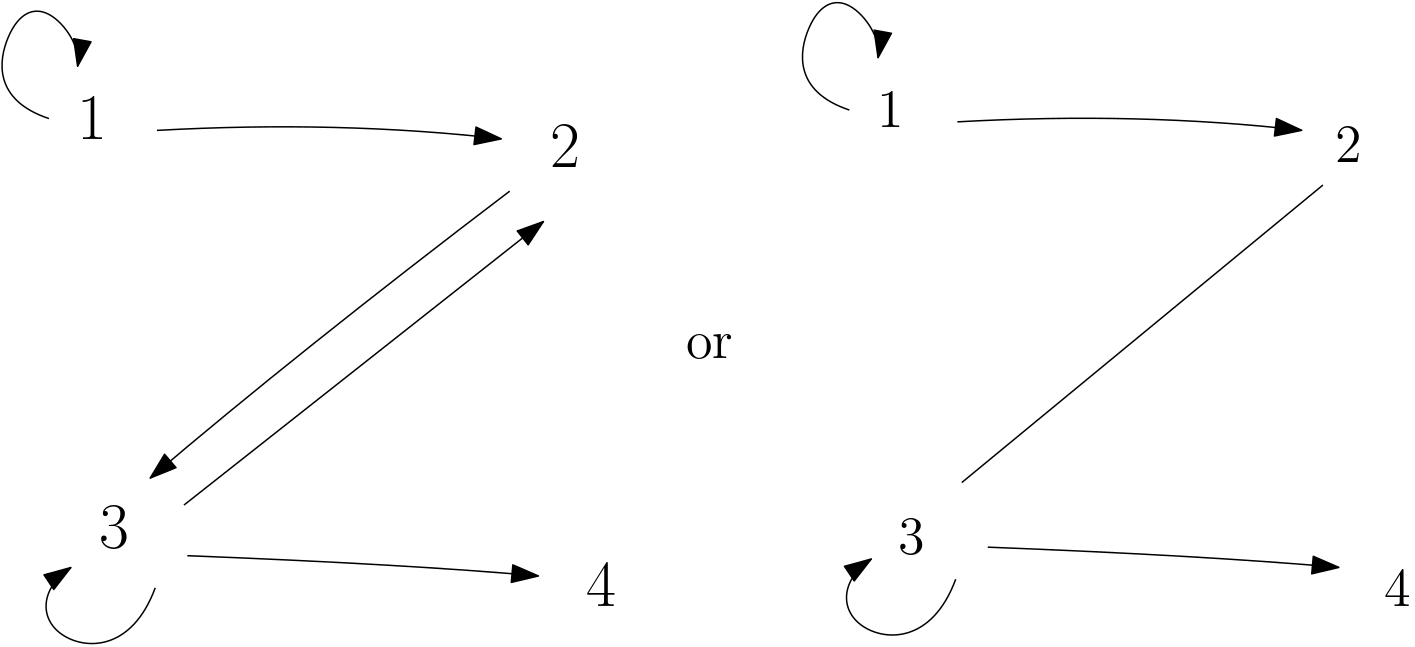
\includegraphics[width=10cm]{graph2.png}
    \end{center}

    The relation matrix $M$ is also called the adjacency matrix of the associated graph.

    \pagebreak

    \emph{Remark.} A relation is reflexive if and only if its directed graph has a loop at each vertex.

    \begin{center}
        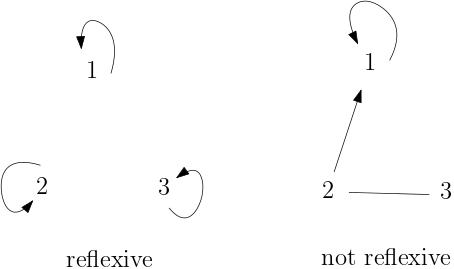
\includegraphics[width=7cm]{graph3.png}
    \end{center}

    \emph{Remark.} A relation is symmetric if and only if its directed graph contains only loops and undirected edges.

    \begin{center}
        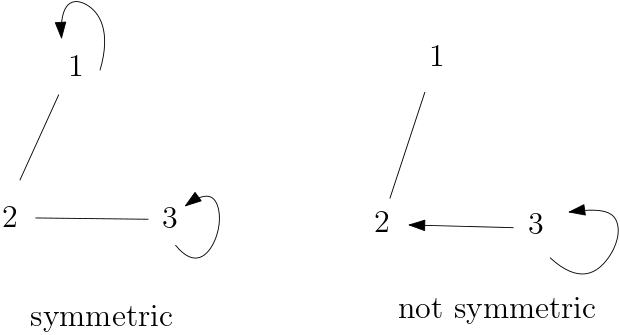
\includegraphics[width=7cm]{graph4.png}
    \end{center}
\end{document}